\documentclass[a4paper, 11pt, twoside]{article}

\usepackage{hyperref}
%\usepackage[ngerman]{babel}
\usepackage[english]{babel}
%\usepackage[latin1]{inputenc}
\usepackage[utf8]{inputenc}

\usepackage{graphicx,float,subfigure}
%\usepackage{pifont}
\usepackage{type1cm}
\usepackage{amssymb, amsthm, amsmath}
\usepackage{listings}

\usepackage{pgf}
\usepackage{url}
%\usepackage{graphicx}
%\usepackage{pifont}
%\usepackage{type1cm}


\usepackage{makeidx}
\makeindex

\setlength{\parindent}{0em}
\setlength{\oddsidemargin}{0.0cm}
\setlength{\evensidemargin}{0.0cm}
\setlength{\textheight}{23cm}
\setlength{\topmargin}{-0.5cm}
\setlength{\footskip}{1.5cm}
\setlength{\textwidth}{15.5cm}

\renewcommand*\familydefault{\sfdefault}

\begin{document}
\thispagestyle{empty}

%\documentclass[a4paper]{article}

%\usepackage{pgf}
%\usepackage{graphicx}
%\usepackage{pifont}
%\usepackage{type1cm}

\setlength{\textwidth}{14cm}
\setlength{\oddsidemargin}{1cm}

%\begin{document}

\thispagestyle{empty}

%%%%%%%%%%%%%%%%%%%%%%%%%%%%%%%%%%%%%%%%
%%%%%%%%%%%%%%%%%%%%%%%%%%%%%%%%%%%%%%%%
%%%%%%%%%%%%%%%%%%%%%%%%%%%%%%%%%%%%%%%%

\newcount \Z
\Z=20

%%% logos %%%

%%% NUMHPC %%%
\newlength{\numhpclogox}
\setlength{\numhpclogox}{\paperwidth} % 20/210ths of the paperwidth
\divide\numhpclogox by 210
\multiply\numhpclogox by 100

\newlength{\numhpclogoy}
\setlength{\numhpclogoy}{\paperheight} % 270/297ths of the paperwidth
\divide \numhpclogoy by 297
\multiply \numhpclogoy by -235

\newlength{\numhpclogoheight}
\setlength{\numhpclogoheight}{\paperheight} % 270/297ths of the paperwidth
\divide\numhpclogoheight by 297
\multiply\numhpclogoheight by 20

%%% KIT %%%
\newlength{\kitlogox}
\setlength{\kitlogox}{\paperwidth} % 20/210ths of the paperwidth
\divide\kitlogox by 210
\multiply\kitlogox by 0

\newlength{\kitlogoy}
\setlength{\kitlogoy}{\paperheight} % 270/297ths of the paperwidth
\divide \kitlogoy by 297
\multiply \kitlogoy by -230

\newlength{\kitlogoheight}
\setlength{\kitlogoheight}{\paperheight} % 270/297ths of the paperwidth
\divide\kitlogoheight by 297
\multiply\kitlogoheight by 15


%%% EMCL %%%
\newlength{\emcllogox}
\setlength{\emcllogox}{\paperwidth} % 20/210ths of the paperwidth
\divide\emcllogox by 210
\multiply\emcllogox by 28

\newlength{\emcllogoy}
\setlength{\emcllogoy}{\paperheight} % 270/297ths of the paperwidth
\divide \emcllogoy by 297
\multiply \emcllogoy by -160

\newlength{\emcllogoheight}
\setlength{\emcllogoheight}{\paperheight} % 270/297ths of the paperwidth
\divide\emcllogoheight by 297
\multiply\emcllogoheight by 20

%%% HIFLOW %%%
\newlength{\hiflowlogox}
\setlength{\hiflowlogox}{\paperwidth} % 20/210ths of the paperwidth
\divide\hiflowlogox by 210
\multiply\hiflowlogox by 28

\newlength{\hiflowlogoy}
\setlength{\hiflowlogoy}{\paperheight} % 270/297ths of the paperwidth
\divide \hiflowlogoy by 297
\multiply \hiflowlogoy by -160

\newlength{\hiflowlogoheight}
\setlength{\hiflowlogoheight}{\paperheight} % 270/297ths of the paperwidth
\divide\hiflowlogoheight by 297
\multiply\hiflowlogoheight by 33

%%%%%%%%%%%%%%%%%%%%%%%%%%%%%%%%%%%%%%%%
%%%%%%%%%%%%%%%%%%%%%%%%%%%%%%%%%%%%%%%%
%%%%%%%%%%%%%%%%%%%%%%%%%%%%%%%%%%%%%%%%

%%% NUMHPC %%%
%%\pgftext[bottom, left, at={\pgfpointadd{\pgfpoint{0pt}{0pt}}{\pgfpoint{\numhpclogox}{\numhpclogoy}}}]{\includegraphics[totalheight=\numhpclogoheight]{numhpc}}

%%% KIT %%%
%%\pgftext[bottom, left, at={\pgfpointadd{\pgfpoint{0pt}{0pt}}{\pgfpoint{\kitlogox}{\kitlogoy}}}]{\includegraphics[totalheight=\kitlogoheight]{kitlogo}}

%%% EMCL %%%
\pgftext[bottom, left, at={\pgfpointadd{\pgfpoint{0pt}{0pt}}{\pgfpoint{\hiflowlogox}{\hiflowlogoy}}}]{
\includegraphics[totalheight=\hiflowlogoheight]{HF3_color}}

%%% horizontal lines %%%
\pgfline{\pgfxy(-1pt,0.1pt)}{\pgfxy(15pt,0.1pt)}
\pgfline{\pgfxy(-1pt,-21.4pt)}{\pgfxy(15pt,-21.4pt)}
%%\pgfline{\pgfxy(-1pt,-22.4pt)}{\pgfxy(15pt,-22.4pt)}

%%% EMCL text %%%
\pgftext[bottom, left, at={\pgfpointadd{\pgfpoint{0pt}{0pt}}{\pgfpoint{0cm}{1cm}}}]{{\LARGE{{\bf Tutorial}}}}

%%% EMCL web %%%
\pgftext[bottom, left, at={\pgfpointadd{\pgfpoint{0pt}{0pt}}{\pgfpoint{10.5cm}{-21.7cm}}}]{{\fontsize{13}{10}\selectfont{} http://www.hiflow3.org/}}

\hspace{2cm}
\begin{picture}(0,0)(-250,-25)

\includegraphics[scale=.22]{emcl.pdf} 
\end{picture}

%%% author %%%
\pgftext[bottom, left, at={\pgfpointadd{\pgfpoint{0pt}{0pt}}{\pgfpoint{0cm}{-4cm}}}]{{
\begin{parbox}{13cm}{
\begin{center}\fontsize{12}{30}\selectfont{} E. Ketelaer, S. Ronn\aa s, A. Helfrich-Schkarbanenko, C. Straub
\end{center}}
\end{parbox}}}

%%% title %%%
\pgftext[bottom, left, at={\pgfpointadd{\pgfpoint{0pt}{0pt}}{\pgfpoint{0cm}{-7.5cm}}}]{{
\begin{parbox}{13cm}{
%%\begin{center}\fontsize{18}{30}\selectfont{} \bf Using HiFlow$^3$ for solving the
\begin{center}\fontsize{22}{30}\selectfont{} \bf Dirichlet Boundary Value Problem\\ for Poisson Equation
\end{center}}
\end{parbox}}}

%%% date %%%
\pgftext[bottom, left, at={\pgfpointadd{\pgfpoint{0pt}{0pt}}{\pgfpoint{0cm}{-16.4cm}}}]{{
\begin{parbox}{13cm}{
\begin{center}\fontsize{12}{24}\selectfont{} 
\vspace{5cm}
\textit{modified on \today}\\ 
\vspace{6.5cm}
\hspace{6cm}\textit{Version 1.3}
\end{center}}
\end{parbox}}}

%fhfh \hfill sjdh

%\end{document}


%\newpage
%\null\newpage

\newcommand{\dd}{\mathrm{d}}
\newtheorem{remark}{Remark}[section]
\thispagestyle{empty}
\tableofcontents

\newpage
\pagestyle{plain}
\framebox[15.5cm]{\parbox[c][2.3cm]{14.0cm}{
{\fontsize{19}{30}\selectfont{} \bf{Applying HiFlow$^3$ for solving the Dirichlet\\ boundary value problem for Poisson equation}
}}}
\vspace{0.5cm}
\section{Introduction}

HiFlow$^3$ is a multi-purpose finite element software providing powerful tools for efficient and accurate solution of a wide range of problems modeled by partial differential equations (PDEs). Based on object-oriented concepts and the full capabilities of C++ the HiFlow$^3$ project follows a modular and generic approach for building efficient parallel numerical solvers. It provides highly capable modules dealing with the mesh setup, finite element spaces, degrees of freedom, linear algebra routines, numerical solvers, and output data for visualization. Parallelism - as the basis for high performance simulations on modern computing systems - is introduced on two levels: coarse-grained parallelism by means of distributed grids and distributed data structures, and fine-grained parallelism by means of platform-optimized linear algebra back-ends.

\subsection{How to Use the Tutorial?}
You find the example code (poisson\_tutorial.cc, poisson\_tutorial.h) and a parameter file for the first numerical example (poisson\_tutorial.xml) in the folder \verb'/hiflow/examples/poisson'. The geometry data (*.inp, *.vtu) is stored in the folder \verb'/hiflow/examples/data'.

\subsubsection{Using HiFlow$^3$ as a Developer}\label{sectiondeveloper}
First build and compile HiFlow$^3$. Go to the directory \verb'/build/example/poisson', where the binary \textbf{poisson\_tutorial} is stored. Type \textbf{./poisson\_tutorial}, to execute the program in sequential mode. To execute in parallel mode \index{program!executing in parallel} with four processes, type \textbf{mpirun -np 4 ./poisson\_tutorial}. In both cases, you need to make sure that the default parameterfile poisson\_tutorial.xml is stored in the same directory as the binary, and that the geometry data specified in the parameter file is stored in \verb'/hiflow/examples/data'. Alternatively, you can specify the path of your own xml-file with the name of your xml-file (first) and the path of your geometry data (second) in the comment line, i.e. \textbf{./poisson\_tutorial} \verb'/"path_to_parameterfile"/"name_of_parameterfile".xml' \verb'/"path_to_geometry_data"/'.


\section{Mathematical Setup}
\subsection{Problem}
Note: For simplification, we explain the mathematical setup only for the two dimensional case. However, it is easy to expand the theory to one or three dimensions. \\
Our aim is solving the Poisson problem with Dirichlet boundary condition\index{boundary condition!Dirichlet} in a domain $\Omega \subset \mathbb{R}^2$ with sufficiently smooth boundary $\partial \Omega$: Find $u\in C^2(\Omega) \cap C_0(\overline{\Omega})$ that satisfies
\begin{eqnarray}\label{poisson_equation}
\begin{array}{rcll}
-\Delta u &=& f, & \text{ in }\Omega,\\
        u &=& 0, & \text{ on }\partial\Omega,
\end{array}
\end{eqnarray}
where $f \in C(\Omega)$ is given. \\

The theory of partial differential equations shows that the computation of classical solutions to (\ref{poisson_equation}) is difficult, see e.g. \cite{evans}. Especially the required assumptions on $u$, $f$ and the general shape of $\Omega$ are causing these difficulties. So we need another form for representing solutions where we only need weaker assumptions on the regularity.

\subsection{Weak Formulation}\label{sectionWeak_formulation}
In the Hilbert space $L^2(\Omega)$ we can re-formulate equation (\ref{poisson_equation}) in a weaker sense. 
Let $u = u(x_1, x_2)$, $f = f(x_1, x_2)$ and $\phi = \phi (x_1, x_2)$.  Find $u \in C_0^2(\Omega)$ such that for all test functions $\varphi\in C_0^\infty(\Omega)$ it holds:

$$\int_\Omega - \Delta u\, \varphi\, \dd x = \int_\Omega f \varphi \dd x\ .$$

Using Green's first identity and the Gaussian integral theorem we get
\begin{eqnarray}\label{var_formulation}
\int_\Omega \nabla u\cdot \nabla\varphi\, \dd x - \int_{\partial\Omega} (\nabla u \cdot n) \varphi(x,y) \dd \sigma = \int_\Omega f \varphi \dd x\ ,
\end{eqnarray}
where $n$ is the (outer) normal vector on $\partial \Omega$. Since the test functions $\varphi$ have compact support in $\Omega$, and therefore $\varphi(x,y)=0$ for $(x,y)\in\partial \Omega$, we get from (\ref{var_formulation}) that
\begin{eqnarray}\label{var_formulation2}
\int_\Omega \nabla u \cdot \nabla\varphi\, \dd x = \int_\Omega f \varphi \dd x \qquad \forall \varphi\in C_0^\infty(\Omega).
\end{eqnarray}
$C_0^\infty(\Omega)$ is dense in the Hilbert space $H^1_0(\Omega)$, or more precisely: Since $\Omega$ is bounded, for any $u \in H^1_0(\Omega)$ there exists a sequence of functions $u_m \in C_0^\infty(\Omega) \cap H^1_0(\Omega)$ such that 
\begin{equation}
u_m \rightarrow u \textit{ in } H^1_0(\Omega).
\end{equation}
(See \cite[Section 5.3.2 Theorem 2]{evans} for further details and the proof). So by approximation, we derive that the identity (\ref{var_formulation2}) holds with the smooth function $\varphi$ replaced by any $\varphi \in H^1_0(\Omega)$. Consequently, the resulting equation makes even sense, i.e. the integrals exist, if we loosen the assumptions on $u$ to $u \in H^1_0(\Omega)$ and those on $f$ to $f \in L^2(\Omega)$. \\
Such an $u$ is called $\mathit{weak}$ solution \index{solution!weak} of (\ref{poisson_equation}).
The bilinear form 
\[
a: H^1_0(\Omega) \times H^1_0(\Omega) \rightarrow \mathbb{R},\quad a(u,\varphi)=\int_\Omega \nabla u \cdot \nabla\varphi\, \dd x  
\]
is continuous and elliptic. The linear form $f: H^1_0(\Omega) \rightarrow \mathbb{R},$ $f(\varphi) = \int_\Omega f\, \varphi\, \dd x$ is continuous, 
see \cite{braess}, Def. 2.4. Therefore, by Lax-Milgram lemma,\index{Lax-Milgram theorem} the problem (\ref{var_formulation2}), i.e. the equation 
\begin{equation}\label{var_formulation2_short}
a(u,\varphi)\ =\ f(\varphi) \quad \forall \varphi \in H^1_0(\Omega), 
\end{equation}
has one and only one solution $u \in H^1_0(\Omega)$, see \cite[Chap 5.8]{gilbarg} or \cite{mclean}\index{solution!uniqueness} \index{solution!existence}. The Cea lemma,\index{Cea lemma} see \cite[Chap. 2.8, 2.5]{brenner}, represents the analogon of the Lax-Milgram theorem for finite dimensional spaces. 
That means, the coercivity of the bilinear form $a$ transfers from $H^1_0(\Omega)$ onto finite dimensional subspace $H_h(\Omega) \subset H^1_0(\Omega)$. 
Hence, equation (\ref{var_formulation2_short}) can be solved by means of the finite element method. 
We use HiFlow$^3$ to find $u_h \in H_h(\Omega)$, which approximates the weak solution $u\in H^1_0(\Omega)$.

\subsection{Classical versus Weak Formulation}
\subsubsection{Assumptions}
If we take a closer look on the assumptions on $u$ and $f$ in the classical and in the weak formulation of the Poisson problem, we can see that in the weak formulation we "got rid" of the hard regularity assumptions on $u$ and $f$. In the variational formulation we only need first derivatives of $u$ and these only in the weak sense. Furthermore, $f$ does not need to be continuous any more but only in $L^2(\Omega)$. \\
One might think that we now are looking for some completely different objects: one with regularity up to $C^2$ and one which only satisfies some identities in the integral sense. But they still are quite similar: If we assume that $f\in L^2(\Omega)$ and $\partial \Omega \in C^2$, then it holds that $u\in H^2(\Omega)$ \cite[Chap 6.3, Theorem 4]{evans}. The imbedding theorem by Sobolev tells us that for $u\in H^2(\Omega)$ exists a representation of $u \in C^0(\Omega)$ \cite[Chap 4]{Adams}. We can even assume lesser regularization for the boundary $\partial \Omega$ to apply the imbedding theorem by Sobolev for elliptic operators, see e.g \cite[Chap 9, Theorem 9.15]{gilbarg} for further reading. Under certain circumstances weak and classical solution even coincide.

\subsubsection{Classical and Weak Solution}
From the derivation in section \ref{sectionWeak_formulation} it is clear that every classical (regular and $C^2(\Omega)$-smooth) solution of (\ref{poisson_equation}) also fulfills (\ref{var_formulation2_short}). So every classical solution is also a weak one. \\
The other way around let $u \in H_0^1(\Omega)$ be a weak solution fulfilling (\ref{var_formulation2_short}). Let furthermore $u \in C^2(\Omega) \cap C_0(\overline{\Omega})$ and additionally $f \in C(\Omega)$. Then it follows that 
\begin{equation}
\int_\Omega f \varphi \dd x = \int_\Omega \nabla u \cdot \nabla\varphi\, \dd x = \int_\Omega - \Delta u \varphi \dd x \qquad \forall \varphi\in C_0^\infty(\Omega) \notag
\end{equation}
and so $u$ is a classical solution because all derivatives are classical ones. \\
So we have some hope to find classical solutions by finding weak solutions which are regular enough but "easier to find".

\subsubsection{$L^2$-Norm, $H^1$-Norm and $H^1$-Seminorm}\label{sectionnorms}
In this section one can see the definitions of the square of the $L^2$-norm, $H^1$-norm and $H^1$-seminorm \cite{evans}, because we compute in section \ref{memberComputeError} the error of our approximation in the $L^2$-norm and $H^1$-seminorm.
\begin{align*}
\Vert u \Vert_{L_2(\Omega)}^2 &:= \int_\Omega \vert u \vert^2 dx, \qquad L^2-\textit{norm}, \\
\vert u \vert_{H^1(\Omega)}^2 &:= \int_\Omega \vert \nabla u \vert^2 dx, \qquad H^1-\textit{seminorm}, \\
\Vert u \Vert_{H^1(\Omega)}^2 &:= \Vert u \Vert_{L_2(\Omega)}^2 + \vert u \vert_{H^1(\Omega)}^2, \qquad H^1-\textit{norm}.
\end{align*}

\section{The Commented Program}
\subsection{Preliminaries}
HiFlow$^3$ is designed for high performance computing on massively parallel machines. 
So it applies the Message Passing Interface (MPI)\index{Message Passing Interface (MPI)}\index{MPI} library specification for message-passing, see sections \ref{sectionmain}, \ref{read-mesh}, \ref{memberComputeError}, \ref{adapt}, \cite{MPI}, \cite{MPIstandard} .\\
The poisson tutorial needs following two input files:
\begin{itemize}
\item A parameter file: The parameter file is an xml-file, which contains all parameters needed to execute the program. It is read in by the program. It is not necessary to recompile the program, when parameters in the xml-file are changed. By default the poisson tutorial reads in the parameter file poisson\_tutorial.xml, see section \ref{sectionparameter file}, which contains the parameters of the first numerical example, see section \ref{sectionfirstexample}.This file is stored in \verb'/hiflow/examples/poisson/'.  
\item Geometry data\index{geometry data}: The file containing the geometry is specified in the parameter file (poisson\_tutorial.xml). In both numerical examples in section \ref{sectionExample} we used \textbf{unit\_square.inp}. You can find different meshes in the folder \verb'/hiflow/examples/data' .
\end{itemize}

HiFlow$^3$ does not generate meshes\index{mesh!generate} for the domain $\Omega$.\index{domain geometry!generating} Meshes in *.inp and *.vtu format can be read in. 
It is possible to extend the reader for other formats.
Furthermore it is possible to generate other geometries by using external programs (Mesh generators) or by hand.\\  

\subsection{Parameter File}\index{parameter file}\label{sectionparameter file}
The parameters required are initialized in the paramter file poisson\_tutorial.xml.
\begin{lstlisting}[language=C++, basicstyle={\footnotesize, \ttfamily}, keywordstyle=\color{blue}, numbers=none, tabsize=4]
<Param>
  <Mesh>
    <Filename1>unit_line.inp</Filename1>
    <Filename2>unit_square.inp</Filename2>
    <Filename3>unit_cube.inp</Filename3>
    <InitialRefLevel>1</InitialRefLevel>
    <FinalRefLevel>8</FinalRefLevel>
    <FeDegree>1</FeDegree>
  </Mesh>
  <LinearAlgebra>
    <NameMatrix>CoupledMatrix</NameMatrix>
    <NameVector>CoupledVector</NameVector>
    <Platform>CPU</Platform>
    <Implementation>Naive</Implementation>
    <MatrixFormat>CSR</MatrixFormat>
  </LinearAlgebra>
  <LinearSolver>
    <Name>CG</Name>
    <SizeBasis>50</SizeBasis>
    <Method>NoPreconditioning</Method>
    <MaxIterations>1000</MaxIterations>
    <AbsTolerance>1.0e-14</AbsTolerance>
    <RelTolerance>1.0e-8</RelTolerance>
    <DivTolerance>1.0e6</DivTolerance>
  </LinearSolver>
</Param>
\end{lstlisting}

\subsection{Structure of the Poisson Tutorial}
Following member functions (signed by \textbullet) are defined in the class poisson\_tutorial. The survey reflects the  access relations between the functions, classes and structs. 
 \begin{itemize}
    \item run()
    \item build\_initial\_mesh()
    \item prepare\_system()
    \begin{itemize}
	\item DirichletZero-struct (poisson\_tutorial.h)
    \end{itemize}
    \item assemble\_system()
    \begin{itemize}
	\item LocalPoissonAssembler-class (poisson\_tutorial.h)
        \begin{itemize}
	    \item ExactSol-struct (poisson\_tutorial.h)
	\end{itemize}    
    \end{itemize}    
    \item solve\_system()
    \item compute\_error()
    \begin{itemize}
	\item L2ErrorIntegrator-class (poisson\_tutorial.h)
	\item H1ErrorIntegrator-class (poisson\_tutorial.h)    
    \end{itemize}  
    \item visualize()
    \item adapt()
 \end{itemize} 
You can find the source text of every member function  in an extra section below. 

%\subsection{Source text variables}
%...

\subsection{Main Function}\index{MPI}\label{sectionmain}
The main function starts the simulation of the Poisson problem (poisson\_tutorial.cc).

\begin{lstlisting}[language=C++, basicstyle={\footnotesize, \ttfamily}, keywordstyle=\color{blue}, numbers=none, tabsize=4]
// Program entry point
int main ( int argc, char** argv )
{
    MPI_Init ( &argc, &argv );

    // set default parameter file
    std::string param_filename ( PARAM_FILENAME );
    std::string path_mesh;
    // if set take parameter file specified on console
    if ( argc > 1 )
    {
        param_filename = std::string ( argv[1] );
    }
    // if set take mesh following path specified on console
    if ( argc > 2 )
    {
        path_mesh = std::string ( argv[2] );
    }
    try
    {
        // Create log files for INFO and DEBUG output
        //std::ofstream info_log("poisson_tutorial_info_log");
        LogKeeper::get_log ( "info" ).set_target ( &( std::cout ) );
        //std::ofstream debug_log("poisson_tutorial_debug_log");
        LogKeeper::get_log ( "debug" ).set_target ( &( std::cout ) );
        std::ofstream error_log ( "poisson_tutorial_error_log" );
        LogKeeper::get_log ( "error" ).set_target ( &( std::cout ) );

        // Create application object and run it
        PoissonTutorial app ( param_filename, path_mesh );
        app.run ( );

    }
    catch ( std::exception& e )
    {
        std::cerr << "\nProgram ended with uncaught exception.\n";
        std::cerr << e.what ( ) << "\n";
        return -1;
    }
    MPI_Finalize ( );
    return 0;
}
\end{lstlisting}

\subsection{Member Functions}
\subsubsection{run()}
The member function run() is defined in the class PoissonTutorial (poisson\_tutorial.cc).

\begin{lstlisting}[language=C++, basicstyle={\footnotesize, \ttfamily}, keywordstyle=\color{blue}, numbers=none, tabsize=4]
// Main algorithm
    void run ( )
    {
        // Construct / read in the initial mesh.
        build_initial_mesh ( );
        // Main adaptation loop.
        while ( !is_done_ )
        {
            // Initialize space and linear algebra.
            prepare_system ( );
            // Compute the stiffness matrix and right-hand side.
            assemble_system ( );
            // Solve the linear system.
            solve_system ( );
            // Compute the error to the exact solution.
            compute_error ( );
            // Visualize the solution and the errors.
            visualize ( );
            adapt ( );
        }
    }
\end{lstlisting}
\newpage
\subsubsection{build\_initial\_mesh()}\index{MPI}\label{read-mesh}
This member function, defined in the class PoissonTutorial, reads the initial mesh (poisson\_tutorial.cc), partitions and distributes mesh if indicated, and writes out the refined mesh of initial refinement level.

\begin{lstlisting}[language=C++, basicstyle={\footnotesize, \ttfamily}, keywordstyle=\color{blue}, numbers=none, tabsize=4]
void PoissonTutorial::build_initial_mesh ( )
{
#ifdef USE_MESH_P4EST
    mesh::IMPL impl = mesh::IMPL_P4EST;
#else
    mesh::IMPL impl = mesh::IMPL_DBVIEW;
#endif

    // Read in the mesh on the master process. The mesh is chosen according to 
    // the dimension of the problem.
    if ( rank_ == MASTER_RANK )
    {
        std::string mesh_name;

        switch ( DIMENSION )
        {
            case 1:
            {
                mesh_name =
                        params_["Mesh"]["Filename1"].get<std::string>
                            ( "unit_line.inp" );
                break;
            }
            case 2:
            {
                mesh_name =
                        params_["Mesh"]["Filename2"].get<std::string>
                            ( "unit_square.inp" );
                break;
            }
            case 3:
            {
                mesh_name =
                        params_["Mesh"]["Filename3"].get<std::string>
                            ( "unit_cube.inp" );
                break;
            }

            default: assert ( 0 );
        }
        std::string mesh_filename;
        if ( path_mesh.empty ( ) )
        {
            mesh_filename = std::string ( DATADIR ) + mesh_name;
        }
        else
        {
            mesh_filename = path_mesh + mesh_name;
        }

        std::vector<MasterSlave> period ( 0, MasterSlave ( 0., 0., 0., 0 ) );

        master_mesh_ = read_mesh_from_file ( mesh_filename, DIMENSION, DIMENSION, 
                                             0, period, impl );

        // Refine the mesh until the initial refinement level is reached.
        const int initial_ref_lvl = params_["Mesh"]["InitialRefLevel"].get<int>( 3 );

        if ( initial_ref_lvl > 0 )
        {
            master_mesh_ = master_mesh_->refine_uniform_seq ( initial_ref_lvl );
        }
        refinement_level_ = initial_ref_lvl;
    }

    // 1D parallel execution is not yet implemented.
    if ( DIMENSION == 1 )
    {
        mesh_ = master_mesh_;
    }
    else
    {
        MPI_Bcast ( &refinement_level_, 1, MPI_INT, MASTER_RANK, comm_ );
        SharedVertexTable shared_verts;

        int uniform_ref_steps;
        mesh_without_ghost_ = partition_and_distribute ( master_mesh_, MASTER_RANK, 
                                                         comm_, &uniform_ref_steps, 
                                                         impl );

        assert ( mesh_without_ghost_ != 0 );
        mesh_ = compute_ghost_cells ( *mesh_without_ghost_, comm_, 
                                      shared_verts, impl );

        // Write out mesh of initial refinement level      
        PVtkWriter writer ( comm_ );
        std::ostringstream name;
        name << "poisson_tutorial_mesh_" << refinement_level_ << ".pvtu";
        std::string output_file = name.str ( );
        writer.add_all_attributes ( *mesh_, true );
        writer.write ( output_file.c_str ( ), *mesh_ );
    }
}
\end{lstlisting}

\textbf{struct DirichletZero} \label{structDirichletZero}\index{boundary condition!modelling}\\
This struct in poisson\_tutorial.h defines the homogeneous Dirichlet boundary condition, given in (\ref{poisson_equation}).
\begin{lstlisting}[language=C++, basicstyle={\footnotesize, \ttfamily}, keywordstyle=\color{blue}, numbers=none, tabsize=4]
// Functor used to impose u = 0 on the boundary.
struct DirichletZero
{
    std::vector<double> evaluate ( const mesh::Entity& face,
                                   const std::vector<Coord>& coords_on_face ) const
    {
        // return array with Dirichlet values for dof:s on boundary face
        return std::vector<double>( coords_on_face.size ( ), 0.0 );
    }
};
\end{lstlisting}

\subsubsection{assemble\_system()}
The member function assemble\_system() computes the stiffness matrix\index{stiffness matrix!assembling} and right-hand side\index{right-hand side!assembling} (poisson\_tutorial.cc). The stiffness matrix, right-hand side vector and solution vector are modified to set correct Dirichlet values for the boundary DoFs.

\begin{lstlisting}[language=C++, basicstyle={\footnotesize, \ttfamily}, keywordstyle=\color{blue}, numbers=none, tabsize=4]
void PoissonTutorial::assemble_system ( )
{
    // Assemble matrix and right-hand-side vector.
    LocalPoissonAssembler<ExactSol> local_asm;
    global_asm_.assemble_matrix ( space_, local_asm, *matrix_ );
    global_asm_.assemble_vector ( space_, local_asm, *rhs_ );

    if ( !dirichlet_dofs_.empty ( ) )
    {
        // Correct Dirichlet dofs.
        matrix_->diagonalize_rows ( vec2ptr ( dirichlet_dofs_ ), 
                                    dirichlet_dofs_.size ( ), 1.0 );
        rhs_->SetValues ( vec2ptr ( dirichlet_dofs_ ), dirichlet_dofs_.size ( ),
                          vec2ptr ( dirichlet_values_ ) );
        sol_->SetValues ( vec2ptr ( dirichlet_dofs_ ), dirichlet_dofs_.size ( ),
                          vec2ptr ( dirichlet_values_ ) );
    }
}
\end{lstlisting} 

\textbf{LocalPoissonAssembler class}\\
This class defined in poisson\_tutorial.h implements the stiffness matrix and right-hand side locally for each cell.

\begin{lstlisting}[language=C++, basicstyle={\footnotesize, \ttfamily}, keywordstyle=\color{blue}, numbers=none, tabsize=4]
// Functor used for the local assembly of the stiffness matrix and load vector.
template<class ExactSol>
class LocalPoissonAssembler : private AssemblyAssistant<DIMENSION, double>
{
  public:

    void operator() ( const Element<double>& element, 
                      const Quadrature<double>& quadrature,
                      LocalMatrix& lm )
    {
        AssemblyAssistant<DIMENSION, double>::initialize_for_element ( element, 
                                                                  quadrature );

        // compute local matrix
        const int num_q = num_quadrature_points ( );
        for ( int q = 0; q < num_q; ++q )
        {
            const double wq = w ( q );
            const int n_dofs = num_dofs ( 0 );
            for ( int i = 0; i < n_dofs; ++i )
            {
                for ( int j = 0; j < n_dofs; ++j )
                {
                    lm ( dof_index ( i, 0 ), dof_index ( j, 0 ) ) +=
                            wq * dot ( grad_phi ( j, q ), grad_phi ( i, q ) ) * 
                            std::abs ( detJ ( q ) );
                }
            }
        }
    }

    void operator() ( const Element<double>& element, 
                      const Quadrature<double>& quadrature,
                      LocalVector& lv )
    {
        AssemblyAssistant<DIMENSION, double>::initialize_for_element ( element, 
                                                                  quadrature );

        const int num_q = num_quadrature_points ( );
        for ( int q = 0; q < num_q; ++q )
        {
            const double wq = w ( q );
            const int n_dofs = num_dofs ( 0 );
            for ( int i = 0; i < n_dofs; ++i )
            {
                lv[dof_index ( i, 0 )] += wq * f ( x ( q ) ) * phi ( i, q ) * 
                     std::abs ( detJ ( q ) );
            }
        }
    }

    double f ( Vec<DIMENSION, double> pt )
    {
        ExactSol sol;
        double rhs_sol;

        switch ( DIMENSION )
        {
            case 1:
            {
                rhs_sol = 4. * M_PI * M_PI * ( M * M ) * sol ( pt );
                break;
            }
            case 2:
            {
                rhs_sol = 4. * M_PI * M_PI * ( M * M + N * N ) * sol ( pt );
                break;
            }
            case 3:
            {
                rhs_sol = 4. * M_PI * M_PI * ( M * M + N * N + O * O ) * 
                      sol ( pt );
                break;
            }
            default: assert ( 0 );
        }

        return rhs_sol;
    }
};
\end{lstlisting}

\textbf{ExactSol struct}\label{structExactSol}\\
The struct ExactSol in poisson\_tutorial.h implements the exact solution \index{solution!exact} $u$ given by (\ref{exactSolution}) and the exact gradient $\nabla u$.

\begin{lstlisting}[language=C++, basicstyle={\footnotesize, \ttfamily}, keywordstyle=\color{blue}, numbers=none, tabsize=4]
struct ExactSol
{

    double operator() ( const Vec<DIMENSION, double>& pt ) const
    {
        const double x = pt[0];
        const double y = ( DIMENSION > 1 ) ? pt[1] : 0;
        const double z = ( DIMENSION > 2 ) ? pt[2] : 0;
        const double pi = M_PI;
        double solution;

        switch ( DIMENSION )
        {
            case 1:
            {
                solution = 10.0 * std::sin ( 2. * M * pi * x );
                break;
            }
            case 2:
            {
                solution = 10.0 * std::sin ( 2. * M * pi * x ) * 
                                  std::sin ( 2. * N * pi * y );
                break;
            }
            case 3:
            {
                solution = 10.0 * std::sin ( 2. * M * pi * x ) * 
                                  std::sin ( 2. * N * pi * y ) * 
                                  std::sin ( 2. * O * pi * z );
                break;
            }

            default: assert ( 0 );
        }
        return solution;
    }

    Vec<DIMENSION, double> eval_grad ( const Vec<DIMENSION, double>& pt ) const
    {
        Vec<DIMENSION, double> grad;
        const double x = pt[0];
        const double y = ( DIMENSION > 1 ) ? pt[1] : 0;
        const double z = ( DIMENSION > 2 ) ? pt[2] : 0;
        const double pi = M_PI;

        switch ( DIMENSION )
        {
            case 1:
            {
                grad[0] = 20. * M * pi * std::cos ( 2. * M * pi * x );
                break;
            }
            case 2:
            {
                grad[0] = 20. * M * pi * std::cos ( 2. * M * pi * x ) *
                        std::sin ( 2. * N * pi * y );
                grad[1] = 20. * N * pi * std::sin ( 2. * M * pi * x ) *
                        std::cos ( 2. * N * pi * y );
                break;
            }
            case 3:
            {
                grad[0] = 20. * M * pi * std::cos ( 2. * M * pi * x ) *
                        std::sin ( 2. * N * pi * y ) * 
                        std::sin ( 2. * O * pi * z );
                grad[1] = 20. * N * pi * std::sin ( 2. * M * pi * x ) *
                        std::cos ( 2. * N * pi * y ) * 
                        std::sin ( 2. * O * pi * z );
                grad[2] = 20. * O * pi * std::sin ( 2. * M * pi * x ) *
                        std::sin ( 2. * N * pi * y ) * 
                        std::cos ( 2. * O * pi * z );
                break;
            }
            default: assert ( 0 );
        }

        return grad;
    }
};
\end{lstlisting}
\subsubsection{solve\_system()}
The member function solve\_system() solves \index{solver} the linear system (poisson\_tutorial.cc). The solver is specified in the parameter file. The poisson equation is symmetric positive definite, which means that CG-method is a good choice, see \ref{sectionparameter file}.

\begin{lstlisting}[language=C++, basicstyle={\footnotesize, \ttfamily}, keywordstyle=\color{blue}, numbers=none, tabsize=4]
void PoissonTutorial::solve_system ( )
{
    LinearSolver<LAD>* solver_;
    LinearSolverFactory<LAD> SolFact;
    solver_ = SolFact.Get (
            params_["LinearSolver"]["Name"].get<std::string>( "CG" ) )->
            params ( params_["LinearSolver"] );
    solver_->SetupOperator ( *matrix_ );
    solver_->Solve ( *rhs_, sol_ );
    delete solver_;
}
\end{lstlisting}

\subsubsection{compute\_error()}\label{memberComputeError}\index{error!computation}\index{MPI}
This member function in poisson\_tutorial.cc computes the error between the approximated and the exact solution mentioned in section \ref{sectionExample} in the $L^2$-norm and $H^1$-seminorm, see section \ref{sectionnorms}.

\begin{lstlisting}[language=C++, basicstyle={\footnotesize, \ttfamily}, keywordstyle=\color{blue}, numbers=none, tabsize=4]
void PoissonTutorial::compute_error ( )
{
    // prepare sol_ for post processing
    sol_->UpdateCouplings ( );

    L2_err_.clear ( );
    H1_err_.clear ( );

    // Compute square of the L2 error on each element, putting the
    // values into L2_err_.
    L2ErrorIntegrator<ExactSol> L2_int ( *( sol_ ) );
    global_asm_.assemble_scalar ( space_, L2_int, L2_err_ );

    // Create attribute with L2 error for output.
    AttributePtr L2_err_attr ( new DoubleAttribute ( L2_err_ ) );
    mesh_->add_attribute ( "L2 error", DIMENSION, L2_err_attr );
    double total_L2_err = std::accumulate ( L2_err_.begin ( ), L2_err_.end ( ), 0. );
    double global_L2_err = 0.;
    MPI_Reduce ( &total_L2_err, &global_L2_err, 1, MPI_DOUBLE, MPI_SUM, MASTER_RANK,
                 comm_ );
    LOG_INFO ( "error", "Local L2 error on partition " << rank_ << " = "
               << std::sqrt ( total_L2_err ) );

    // Compute square of the H1 error on each element, putting the
    // values into H1_err_.

    H1ErrorIntegrator<ExactSol> H1_int ( *( sol_ ) );
    global_asm_.assemble_scalar ( space_, H1_int, H1_err_ );

    // Create attribute with H1 error for output.
    AttributePtr H1_err_attr ( new DoubleAttribute ( H1_err_ ) );
    mesh_->add_attribute ( "H1 error", DIMENSION, H1_err_attr );
    double total_H1_err = std::accumulate ( H1_err_.begin ( ), H1_err_.end ( ), 0. );
    double global_H1_err = 0.;
    MPI_Reduce ( &total_H1_err, &global_H1_err, 1, MPI_DOUBLE, MPI_SUM, MASTER_RANK,
                 comm_ );
    LOG_INFO ( "error", "Local H1 error on partition " << rank_ << " = "
               << std::sqrt ( total_H1_err ) );

    if ( rank_ == MASTER_RANK )
    {
        std::cout << "Global L2 error = " << std::sqrt ( global_L2_err ) << "\n"
                << "Global H1 error = " << std::sqrt ( global_H1_err ) << "\n";
    }
}
\end{lstlisting}

\textbf{L2ErrorIntegrator class}\\
The class L2ErrorIntegrator implements the evaluation of the square of the $L^2$-norm of the error on each element (poisson\_tutorial.h).

\begin{lstlisting}[language=C++, basicstyle={\footnotesize, \ttfamily}, keywordstyle=\color{blue}, numbers=none, tabsize=4]
template<class ExactSol>
class L2ErrorIntegrator : private AssemblyAssistant<DIMENSION, double>
{
  public:

    L2ErrorIntegrator ( CoupledVector<Scalar>& pp_sol )
    : pp_sol_ ( pp_sol )
    {
    }

    void operator() ( const Element<double>& element, 
                      const Quadrature<double>& quadrature,
                      double& value )
    {
        AssemblyAssistant<DIMENSION, double>::initialize_for_element ( element, 
                                                                   quadrature );

        // Evaluate the computed solution at all quadrature points.
        evaluate_fe_function ( pp_sol_, 0, approx_sol_ );

        const int num_q = num_quadrature_points ( );
        for ( int q = 0; q < num_q; ++q )
        {
            const double wq = w ( q );
            const double delta = sol_ ( x ( q ) ) - approx_sol_[q];
            value += wq * delta * delta * std::abs ( detJ ( q ) );
        }
    }

  private:
    // coefficients of the computed solution
    const CoupledVector<Scalar>& pp_sol_;
    // functor to evaluate exact solution
    ExactSol sol_;
    // vector with values of computed solution evaluated
    // at each quadrature point
    FunctionValues< double > approx_sol_;
};
\end{lstlisting}

\textbf{H1ErrorIntegrator class}\\
The class H1ErrorIntegrator implements the evaluation of the square of the $H^1$-seminorm of the error on each element (poisson\_tutorial.h).

\begin{lstlisting}[language=C++, basicstyle={\footnotesize, \ttfamily}, keywordstyle=\color{blue}, numbers=none, tabsize=4]
template<class ExactSol>
class H1ErrorIntegrator : private AssemblyAssistant<DIMENSION, double>
{
  public:

    H1ErrorIntegrator ( CoupledVector<Scalar>& pp_sol )
    : pp_sol_ ( pp_sol )
    {
    }

    void operator() ( const Element<double>& element, 
                      const Quadrature<double>& quadrature,
                      double& value )
    {
        AssemblyAssistant<DIMENSION, double>::initialize_for_element ( element, 
                                                                   quadrature );

        // Evaluate the gradient of the computed solution 
        // at all quadrature points.
        evaluate_fe_function_gradients ( pp_sol_, 0, approx_grad_u_ );

        const int num_q = num_quadrature_points ( );
        for ( int q = 0; q < num_q; ++q )
        {
            const Vec<DIMENSION, double> grad_u = sol_.eval_grad ( x ( q ) );
            value += w ( q ) * ( dot ( grad_u, grad_u )
                    - 2. * dot ( grad_u, approx_grad_u_[q] )
                    + dot ( approx_grad_u_[q], approx_grad_u_[q] ) )
                    * std::abs ( detJ ( q ) );
        }
    }

  private:
    // coefficients of the computed solution
    const CoupledVector<Scalar>& pp_sol_;
    // functor to evaluate exact solution
    ExactSol sol_;
    // gradient of computed solution evaluated
    // at each quadrature point
    FunctionValues< Vec<DIMENSION, double> > approx_grad_u_;
};
\end{lstlisting}
%
%

\subsubsection{visualize()}\label{sec:visualize}
The member function visualize() in poisson\_tutorial.cc writes out data for visualization. Note that HiFlow$^3$ has no own visualising module \index{visualization} , so far.

\begin{lstlisting}[language=C++, basicstyle={\footnotesize, \ttfamily}, keywordstyle=\color{blue}, numbers=none, tabsize=4]
void PoissonTutorial::visualize ( )
{
    // Setup visualization object.
    int num_intervals = 2;
    ParallelCellVisualization<double> visu ( space_, num_intervals, comm_, 
                                             MASTER_RANK );

    // Generate filename.
    std::stringstream name;
    name << "solution" << refinement_level_;

    std::vector<double> remote_index ( mesh_->num_entities ( mesh_->tdim ( ) ), 
                                       0 );
    std::vector<double> sub_domain ( mesh_->num_entities ( mesh_->tdim ( ) ), 
                                     0 );
    std::vector<double> material_number ( mesh_->num_entities ( mesh_->tdim ( ) ), 
                                          0 );

    for ( mesh::EntityIterator it = mesh_->begin ( mesh_->tdim ( ) );
          it != mesh_->end ( mesh_->tdim ( ) );
          ++it )
    {
        int temp1, temp2;
        if ( DIMENSION > 1 )
        {
            mesh_->get_attribute_value ( "_remote_index_", mesh_->tdim ( ),
                                         it->index ( ),
                                         &temp1 );
            mesh_->get_attribute_value ( "_sub_domain_", mesh_->tdim ( ),
                                         it->index ( ),
                                         &temp2 );
            remote_index.at ( it->index ( ) ) = temp1;
            sub_domain.at ( it->index ( ) ) = temp2;
        }
        material_number.at ( it->index ( ) ) = 
            mesh_->get_material_number ( mesh_->tdim ( ), it->index ( ) );
    }

    visu.visualize ( EvalFeFunction<LAD>( space_, *( sol_ ) ), "u" );

    // visualize error measures
    visu.visualize_cell_data ( L2_err_, "L2" );
    visu.visualize_cell_data ( H1_err_, "H1" );
    visu.visualize_cell_data ( remote_index, "_remote_index_" );
    visu.visualize_cell_data ( sub_domain, "_sub_domain_" );
    visu.visualize_cell_data ( material_number, "Material Id" );
    visu.write ( name.str ( ) );
}
\end{lstlisting}

\subsubsection{adapt()}\index{MPI}\label{adapt}
The member function adapt() modifies the space through refinement\index{mesh!adapt}\index{mesh!refine} (poisson\_tutorial.cc). 

\begin{lstlisting}[language=C++, basicstyle={\footnotesize, \ttfamily}, keywordstyle=\color{blue}, numbers=none, tabsize=4]
void PoissonTutorial::adapt ( )
{
    // Refine mesh on master process. 1D parallel execution is 
    // not yet implemented.
    if ( DIMENSION == 1 )
    {
        if ( rank_ == MASTER_RANK )
        {
            const int final_ref_level = params_["Mesh"]["FinalRefLevel"].
                  get<int>( 6 );
            if ( refinement_level_ >= final_ref_level )
            {
                is_done_ = true;
            }
            else
            {
                mesh_ = mesh_->refine ( );
                ++refinement_level_;
            }
        }
    }
    else
    {
#ifdef USE_MESH_P4EST
        const int final_ref_level = params_["Mesh"]["FinalRefLevel"].
             get<int>( 6 );
        if ( refinement_level_ >= final_ref_level )
        {
            is_done_ = true;
        }
        else
        {
            mesh_without_ghost_ = mesh_without_ghost_->refine ( );
            ++refinement_level_;
        }
        if ( !is_done_ )
        {
            SharedVertexTable shared_verts;
            std::vector<MasterSlave> period ( 0, MasterSlave ( 0., 0., 0., 0 ) );
            mesh_ = compute_ghost_cells ( *mesh_without_ghost_, comm_, 
                                          shared_verts, mesh::IMPL_P4EST );
        }
#else
#    ifdef WITH_PARMETIS
        const int final_ref_level = params_["Mesh"]["FinalRefLevel"].
              get<int>( 6 );
        if ( refinement_level_ >= final_ref_level )
        {
            is_done_ = true;
        }
        else
        {
            mesh_without_ghost_ = mesh_without_ghost_->refine ( );
            ++refinement_level_;
        }

        if ( !is_done_ )
        {
            // Repartition the new mesh.
            ParMetisGraphPartitioner parmetis_partitioner;
            MeshPtr local_mesh = repartition_mesh ( mesh_without_ghost_, comm_, 
                                                    &parmetis_partitioner );
            assert ( local_mesh != 0 );
            mesh_.reset ( );
            SharedVertexTable shared_verts;
            mesh_ = compute_ghost_cells ( *local_mesh, comm_, shared_verts );
            local_mesh.reset ( );
        }
#    else
        if ( rank_ == MASTER_RANK )
        {
            const int final_ref_level = params_["Mesh"]["FinalRefLevel"].
                     get<int>( 6 );
            if ( refinement_level_ >= final_ref_level )
            {
                is_done_ = true;
            }
            else
            {
                master_mesh_ = master_mesh_->refine ( );
                ++refinement_level_;
            }
        }
        // Broadcast information from master to slaves.
        MPI_Bcast ( &refinement_level_, 1, MPI_INT, MASTER_RANK, comm_ );
        MPI_Bcast ( &is_done_, 1, MPI_CHAR, MASTER_RANK, comm_ );

        if ( !is_done_ )
        {
            // Distribute the new mesh.
            MeshPtr local_mesh = partition_and_distribute ( master_mesh_, 
                                                            MASTER_RANK, 
                                                            comm_ );
            assert ( local_mesh != 0 );
            SharedVertexTable shared_verts;
            mesh_ = compute_ghost_cells ( *local_mesh, comm_, shared_verts );
        }
#    endif
#endif
        PVtkWriter writer ( comm_ );
        std::ostringstream name;
        name << "poisson_tutorial_mesh_" << refinement_level_ << ".pvtu";
        std::string output_file = name.str ( );
        writer.add_all_attributes ( *mesh_, true );
        writer.write ( output_file.c_str ( ), *mesh_ );
    }
}
\end{lstlisting}

\section{Program Output}
HiFlow$^3$ can be executed in a parallel or sequential mode which influence the generated output data. Note that the log files can be viewed by any editor.
\subsection{Parallel Mode} \index{parallel mode}
Executing the program in parallel, for example with four processes by \textbf{mpirun -np 4 ./poisson\_tutorial}  \index{program!executing in parallel} 
generates following output data. 
\begin{itemize}
\item Mesh/geometry data:
\begin{itemize}
\item \textbf{poisson\_tutorial\_mesh.pvtu} Global mesh of initial refinement level with default value = 3 (parallel vtk-format). It combines the local meshes of sequential vtk-format owned by the different processes to the global mesh.
\item \textbf{poisson\_tutorial\_mesh\_X.vtu} local mesh of initial refinement level (default value = 3) owned by process X for X=0, 1, 2 and 3 (vtk-format).
\end{itemize}
\item Solution data:
\begin{itemize}
\item \textbf{solutionX.pvtu} Solution of the poisson problem for refinement level X=3, 4, 5, 6, 7 and 8  (parallel vtk-format). It combines the local solutions owned by the different processes to a global solution.
\item \textbf{solutionX\_Y.vtu} Local solution of the poisson problem for refinement level X=3, 4, 5, 6, 7 and 8 of the degrees of freedoms which belong to cells owned by process Y, for Y=0, 1, 2 and 3 (vtk-format).
\end{itemize}
\item Log files:
\begin{itemize}
\item \textbf{poisson\_tutorial\_debug\_log} Log file listing errors helping to simplify the debugging process. This file is empty if the program runs without errors.
\item \textbf{poisson\_tutorial\_info\_log} Log file listing parameters and some helpful information to control 
      the program as for example information about the residual of the linear and non-linear solver used.
\end{itemize}
\item Terminal output: The global errors in $L^2$-norm and $H^1$-seminorm are listed for the different refinement levels. 
\end{itemize}

\subsection{Sequential Mode} \index{sequential mode}
Executing the program sequentially by \textbf{./poisson\_tutorial} following output data is generated.\index{program!executing sequentially} 
\begin{itemize}
\item Mesh/geometry data:
\begin{itemize}
\item \textbf{poisson\_tutorial\_mesh.pvtu} Global mesh (parallel vtk-format). 
\item \textbf{poisson\_tutorial\_mesh\_0.vtu} Global mesh owned by process 0 (vtk-format) containing the mesh information.
\end{itemize}
\item Solution data. 
\begin{itemize}
\item \textbf{solutionX.vtu} Solution of the poisson problem for refinement level X=3, 4, 5, 6, 7 and 8 (vtk-format). 
\end{itemize}
\item Log files:
\begin{itemize}
\item \textbf{poisson\_tutorial\_debug\_log} is a list of errors helping to simplify the debugging process. This file keeps empty if the program runs without errors.
\item \textbf{poisson\_tutorial\_info\_log} is a list of parameters and some helpful informations to control the program as for example information 
                                         about the residual of the linear and non-linear solver used.
\end{itemize}
\item Terminal output: The global errors in $L^2$-norm and $H^1$-seminorm are listed for the different refinement levels. 
\end{itemize}

\subsection{Visualizing the Solution}
HiFlow$^3$ only generates output data, see section \ref{sec:visualize}, but does not visualize. The mesh/geometry data as well as the solution data can be visualized 
by any external program which can handle the vtk data format as e.g. the program paraview \cite{Paraview}.\index{paraview} 



\section{Examples}\label{sectionExample}
\subsection{First Example}\label{sectionfirstexample}

This example is implemented in one to three dimensions. All three cases are discussed in the following.
\subsubsection{One Dimension}\label{sectiononedimension}
To be able to verify the results  we choose in this example the right-hand side 
\begin{equation}
f(x,y)\ =\ 4 \pi^2 M^2 \sin(2 \pi M x )  \text{ with } M\in \mathbb{N}, 
\end{equation}
and the homogeneous Dirichlet data on the boundary of the unit line $\Omega:=(0,1)$. The analytical solution is obviously
\begin{equation}\label{exactSolution}
u(x,y)\ =\ \sin(2 \pi M x ).  
\end{equation}
Obviously, $u \in C^2(\Omega) \cap C_0(\overline{\Omega})$ holds since $\sin$ is an analytic function.
Considering $u$ and $f$ we see that $u$ is an eigenfunction of the operator $- \Delta u$ on $\Omega$ with the eigenvalue $4 \pi^2 M^2$. \\
Hence, the error in the $L^2$-norm $\Vert u-u_h \Vert_{L^2(\Omega)}$ as well as the error in the $H^1$-seminorm $\vert u-u_h \vert_{H^1(\Omega)}$ between the finite element approximation and the exact solution
can be computed, see section \ref{memberComputeError}.\index{error} Similar results can be shown for the two dimension and the three dimension case.
Fig. \ref{1dsol4} - \ref{1dsol8} show the visualized solution for refinement level 4, 6 and 8 for $M=4$.


\begin{figure}[h!]
	\centering
		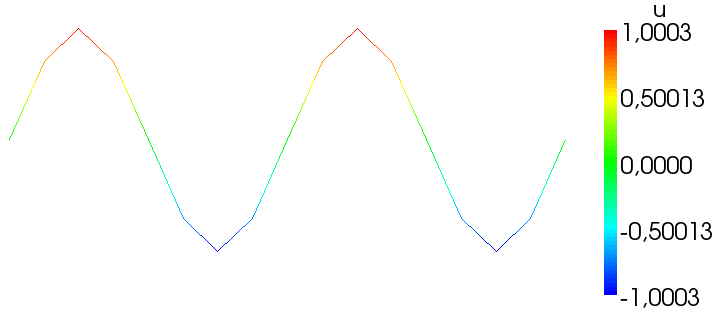
\includegraphics[width=0.45\textwidth]{fig/u_poisson_tut_1d_lvl4_M2_trans.png}
\caption{Global solution in 1D for refinement level 4 of the mesh.}
\label{1dsol4}
\end{figure}

\begin{figure}[h!]
	\centering
		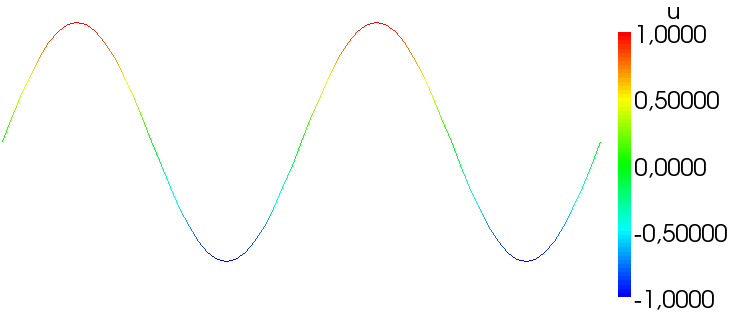
\includegraphics[width=0.45\textwidth]{fig/u_poisson_tut_1d_lvl6_M2_trans.png}
\caption{Global solution in 1D for refinement level 6 of the mesh.}
\label{1dsol6}
\end{figure}

\begin{figure}[h!]
	\centering
		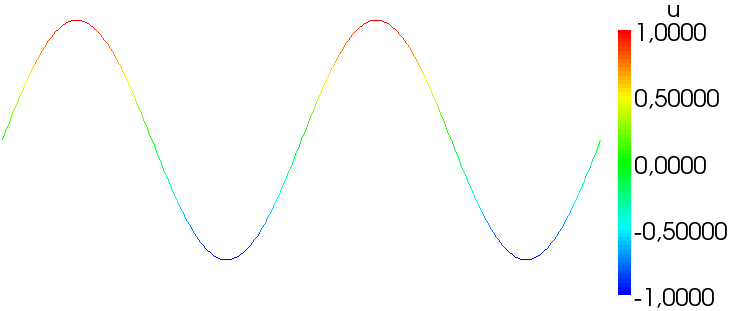
\includegraphics[width=0.45\textwidth]{fig/u_poisson_tut_1d_lvl8_M2_trans.png}
\caption{Global solution in 1D for refinement level 8 of the mesh.}
\label{1dsol8}
\end{figure}

\newpage

\subsubsection{Two Dimensions}\label{sectiontwodimensions}
We expand the right-hand side to two dimensions, i.e.
\begin{equation}
f(x,y)\ =\ 4 \pi^2 (M^2 + N^2) \sin(2 \pi M x ) \sin(2 \pi N y) \text{ with } M,N\in \mathbb{N}, 
\end{equation}
and choose again homogeneous Dirichlet data on the boundary. $\Omega$ is now the unit square $\Omega:=(0,1)\times(0,1)$. By means of the separation methods we derive the analytical solution 
\begin{equation}\label{exactSolution}
u(x,y)\ =\ \sin(2 \pi M x ) \sin(2 \pi N y).  
\end{equation}


Fig. \ref{2dsol4} - \ref{2dsol8} show the visualized solution for refinement level 4, 6 and 8 for $M=2$ and $N=4$. On the right side the corresponding mesh is included in the picture.
\begin{figure}[h!]
	\centering
	\subfigure[Solution.]{
		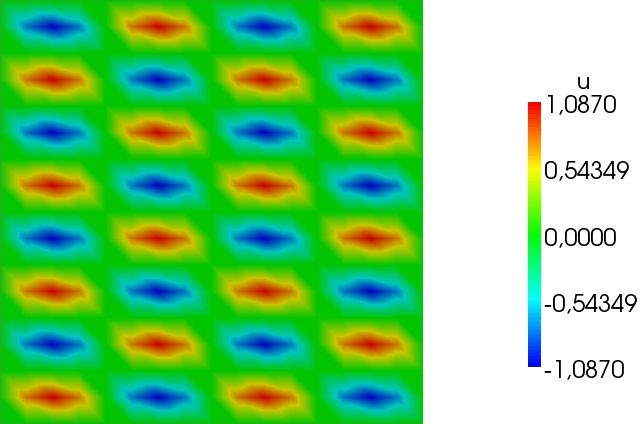
\includegraphics[width=0.45\textwidth]{fig/u_poisson_tut_lvl4_M2N4_trans.png}
	}
	\subfigure[Solution with mesh.]{
		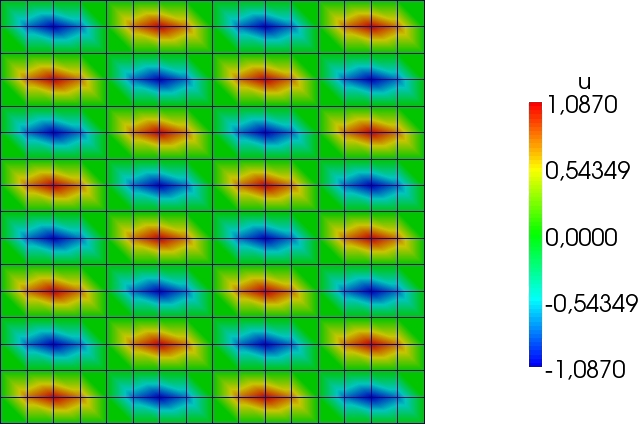
\includegraphics[width=0.45\textwidth]{fig/u_poisson_tut_lvl4_M2N4_mesh_trans.png}
	}
\caption{Global solution in 2D for refinement level 4 of the mesh.}
\label{2dsol4}
\end{figure}

\begin{figure}[h!]
	\centering
	\subfigure[Solution.]{
		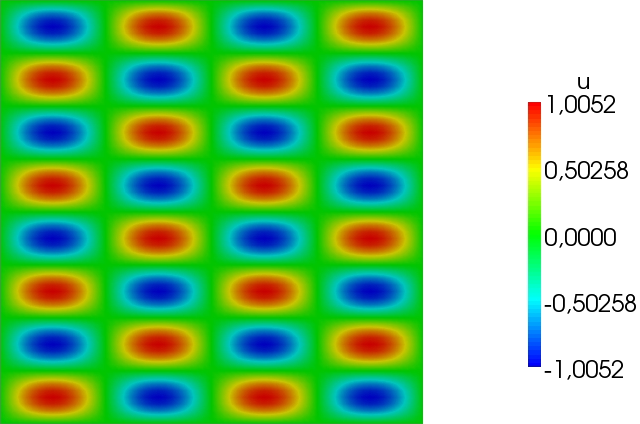
\includegraphics[width=0.45\textwidth]{fig/u_poisson_tut_lvl6_M2N4_trans.png}
	}
	\subfigure[Solution with mesh.]{
		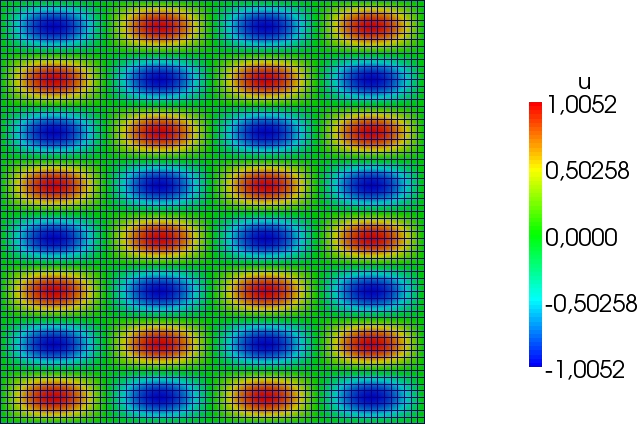
\includegraphics[width=0.45\textwidth]{fig/u_poisson_tut_lvl6_M2N4_mesh_trans.png}
	}
\caption{Global solution in 2D for refinement level 6 of the mesh.}
\label{2dsol6}
\end{figure}

\begin{figure}[h!]
	\centering
	\subfigure[Solution.]{
		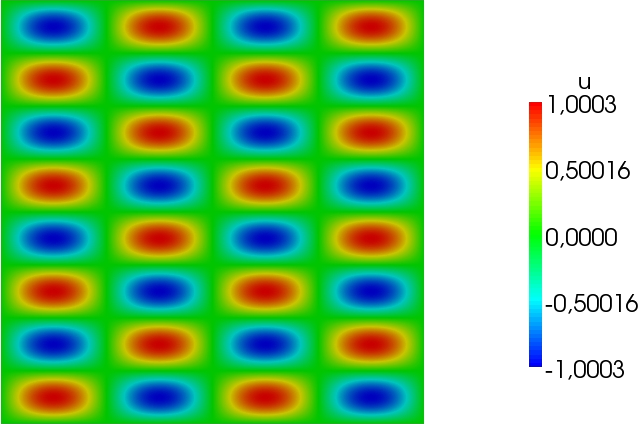
\includegraphics[width=0.45\textwidth]{fig/u_poisson_tut_lvl8_M2N4_trans.png}
	}
	\subfigure[Solution with mesh.]{
		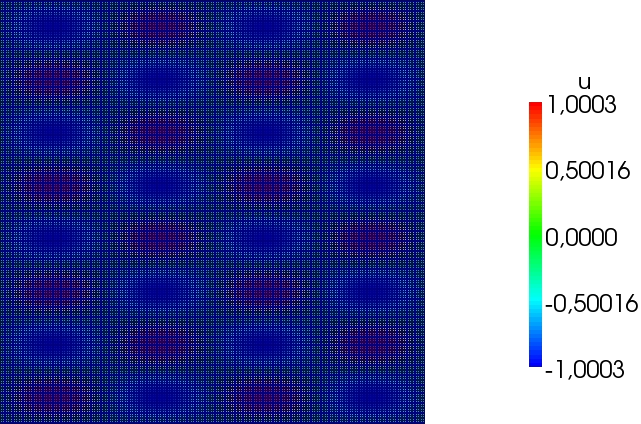
\includegraphics[width=0.45\textwidth]{fig/u_poisson_tut_lvl8_M2N4_mesh_trans.png}
	}
\caption{Global solution in 2D for refinement level 8 of the mesh.}
\label{2dsol8}
\end{figure}



\subsubsection{Three Dimensions}\label{sectionthreedimensions}
Now we do the same thing for three dimensions. The right-hand side changes to
\begin{equation}
f(x,y,z)\ =\ 4 \pi^2 (M^2 + N^2 + O^2) \sin(2 \pi M x ) \sin(2 \pi N y) \sin(2 \pi O z ) \text{ with } M,N,O \in \mathbb{N}, 
\end{equation}
$\Omega$ is now the unit cube $\Omega:=(0,1)\times(0,1)\times(0,1)$. Again, by means of the separation methods we derive the analytical solution 
\begin{equation}\label{exactSolution}
u(x,y)\ =\ \sin(2 \pi M x ) \sin(2 \pi N y) \sin(2 \pi O z).  
\end{equation}

Fig. \ref{3dsol3} and \ref{3dsol5} show the visualized solution for refinement levels 3 and 5 for $M=4$, $N=2$ and $O=1$, including the corresponding mesh.

\begin{figure}[h!]
	\centering
		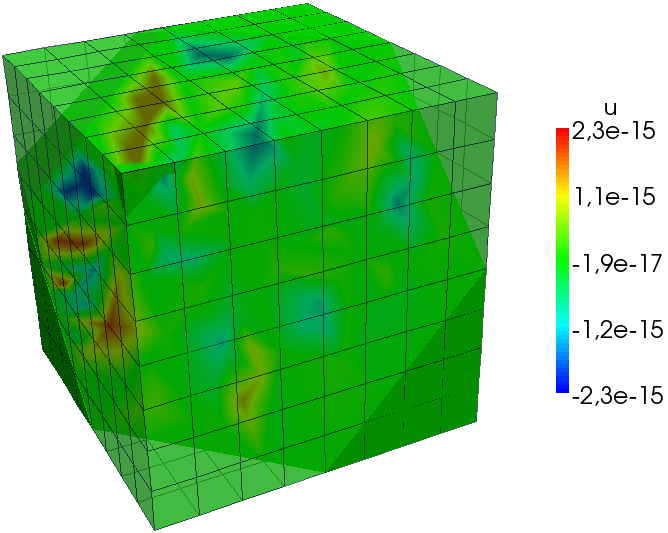
\includegraphics[width=0.45\textwidth]{fig/u_poisson_tut_3d_lvl3_M2N4O1_mesh_trans.png}
\caption{Global solution in 3D for refinement level 3 of the mesh.}
\label{3dsol3}
\end{figure}

\begin{figure}[h!]
	\centering
		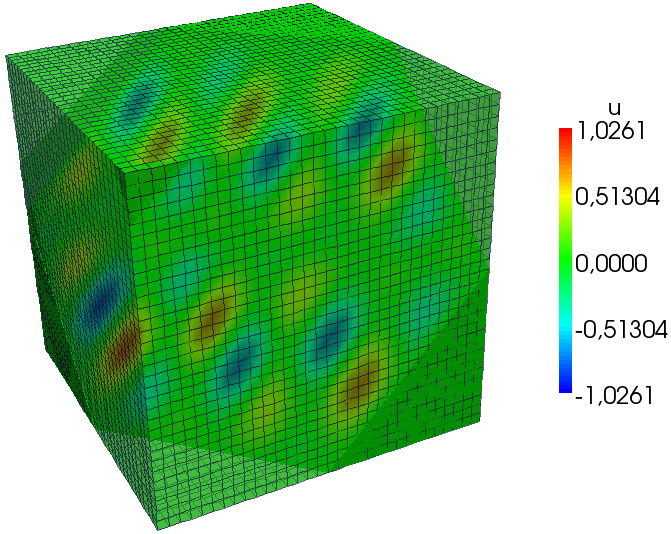
\includegraphics[width=0.45\textwidth]{fig/u_poisson_tut_3d_lvl5_M2N4O1_mesh_trans.png}
\caption{Global solution in 3D for refinement level 5 of the mesh.}
\label{3dsol5}
\end{figure}



\newpage

\subsection{Second Example}\label{section:second_example}
Now we take a look on a second example in two dimensions, where we change the right-hand side $f$ to
\begin{equation}
f(x,y) = 32[x(1-x) + y(1-y)]. \notag
\end{equation}
In this case, the exact solution to the Poisson problem (\ref{poisson_equation}) is given by
\begin{equation}
u(x,y) = 16x(1-x)y(1-y).
\label{example2}
\end{equation}
Obviously, $u$ is eigenfunction of the Laplace operator on a square $\Omega$. In contrast to the first example the solution computed on the fine grid with 1024 elements in (\ref{polynom}) looks perfectly smooth. The reason for this observation lies in the nature of the solution: the solution $u$ given by (\ref{example2}) is a polynomial of second order and does not oscillate as much as the solution in the first example. The solution in this example can be interpolated much better and more accurate by linear elements than the solution in the first example. \\
\begin{figure}[htb]
  \centering      
  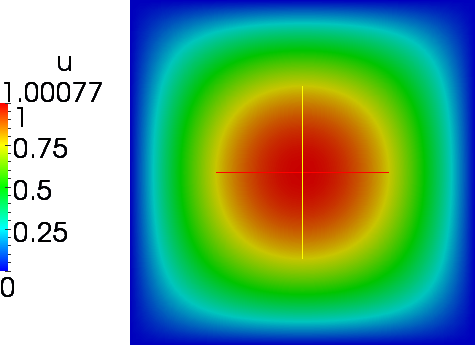
\includegraphics[width=0.45\textwidth]{fig/polynom_trans.png}
\caption{Global solution for refinement level 5 of the mesh for the second example.}
\label{polynom}
\end{figure}
Our expectation is that increasing the polynomial degree of the ansatz functions affects the quality of the approximation less in the second example as in the first one. The dependence upon the parameters polynomial degree $p$ and level of refinement, measured by the quantity $h$, will be investigated in the next section.

\section{Quality of the Approximation}
An important aspect of the finite element method is that it approximates the space in which we are looking for the exact solution to the weak formulation of the partial differential equation, i.e. in our case $H_0^1(\Omega)$. Compared the the finite difference method where you approximate the occuring derivatives by difference quotients it is a completely different approach which affects practical aspects:
\begin{itemize}
\item We can now connect the approximating subspace to the discretization of the domain $\Omega$ and vice versa.
\item As a consequence, the approximating subspace is customized to the domain so that we have the flexibility to handle complex domains.
\item A good choice of the discretization of $\Omega$ can improve the quality of the approximation significantly.
\end{itemize}

For our case of conforming elements and piecewise polynomial basis functions this naturally leads to two parameters which we can vary to get a better approximation $u_h \in H_h(\Omega)\subset H^1_0(\Omega)$.

\subsection{Convergence Theory}
We want that the solution $u_h$ converges in some sense to the exact solution of the infinite dimensional weak problem. In the case of the finite element method with conforming Lagrangian ansatz functions, there are two parameters that we can vary:
\begin{itemize}
\item The fineness of the grid which is measured by
\begin{equation}
h := \max_{K \in \mathcal{T}^h} diam K, \notag
\end{equation}
where $\mathcal{T}^h$ denotes the set of all elements $K$ in the triangulation.
\item The polynomial degree $p$ of the Lagrangian ansatz functions.
\end{itemize}
We can expect that the errors in the approximation depend on these parameters, and that the quality of the approximation can somehow be measured in dependence of them. Cea lemma  gives us an error estimate reduced to an interpolation estimate
\begin{equation}
\Vert u-u_h\Vert_X \leq C \inf_{v_h \in X_h} \Vert u-v_h\Vert_X \leq C \Vert u-I_hu \Vert_X, \notag
\end{equation}
where $X=H_0^1(\Omega)$ and $X^h \subset X$ is the conforming finite element space and $I_h$ denotes the interpolation operator. \\
Furthermore, it can be shown that 
\begin{equation}
\Vert u-I_hu\Vert_{L^2} \leq C h^{p+1} \Vert u\Vert_{H^{p+1}}, \quad \Vert \nabla (u-I_hu)\Vert_{L^2} \leq C h^p \Vert u\Vert_{H^{p+1}}, 
\end{equation}
see e.g. \cite{braess}.

\subsection{Dependence on $h$}
First, we want to anticipate that in both examples the approximate solution converges with increasing refinement level to the exact solution. But the interesting question is about the differences how they converge.
\subsubsection{First Example}
For this experiment we fixed the polynomial degree to $1$, i.e. we used linear elements, we worked in two dimensions and refined the grid up to six times. For the parameters we chose the case $M=N=1$. The global error in the $L^2$-norm and in the $H^1$-norm is plotted in fig. \ref{error_DOF_example1}. For the number of degrees of freedom we chose a logarithmic scale, because with each refinement step the number of degrees of freedom increases exponentially. \\
\begin{figure}[htb]
  \centering      
  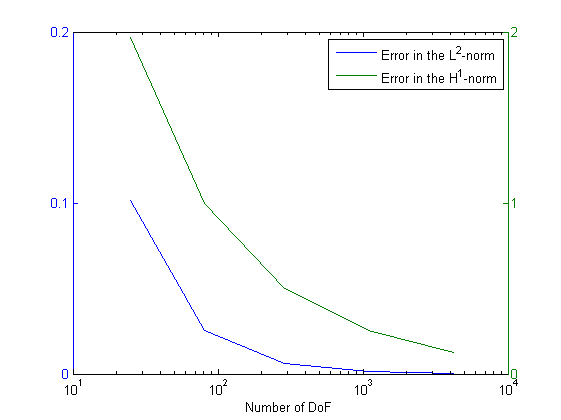
\includegraphics[width=0.65\textwidth]{fig/errorf1.png}
\caption{Global error in the $L^2$- and $H^1$-norm as function of the number of DoF for polynomial degree $1$ for $M = N = 1$.}
\label{error_DOF_example1}
\end{figure}
In fig. \ref{error_DOF_example1}, one can clearly see the expected quadratic behaviour in the $h$ dependence which leads to a quick decrease of the error in the $L^2$-norm. Also in the plot of the error in the $H^1$-norm, the expected linear decrease with respect to $h$ can be seen. This especially means that the error in the gradient dominates the error in the full $H^1$-norm.
\subsubsection{Second Example}
The plot of the global error in the $L^2$- and $H^1$-norm for the second example from section \ref{section:second_example} can be seen in fig. \ref{H^1_error_example2}. The plot configurations are the same as in the first example, i.e. we chose a logarithmic scale for the number of degrees of freedom.
\begin{figure}[htb]
  \centering      
  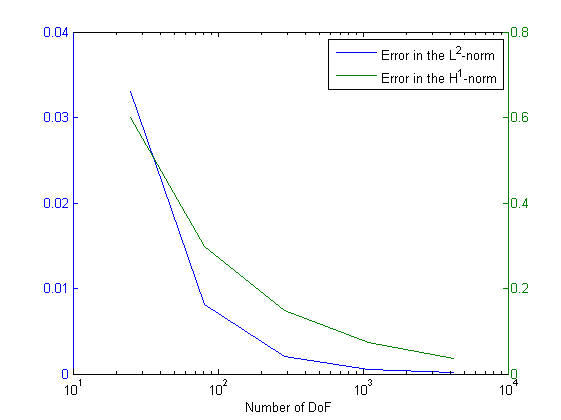
\includegraphics[width=0.65\textwidth]{fig/errorf2.png}
\caption{Global error in the $L^2$- and $H^1$-norm as function of the number of DoF for polynomial degree 1 for the second example.}
\label{H^1_error_example2}
\end{figure}
The observations in this example are quite the same as in the first. Especially the plot matches with our expectations about the decrease of the errors.

\subsection{Dependence on the Polynomial Degree $p$}
\subsubsection{First Example}
For the experiments within this section, we keep the mesh fixed and the polynomial degree is increased, see fig. \ref{error_polydegree_example1}. For this experiment we chose a constant refinement level of three, i.e. $h=\frac{1}{8}$.
\begin{figure}[h!]
  \centering      
  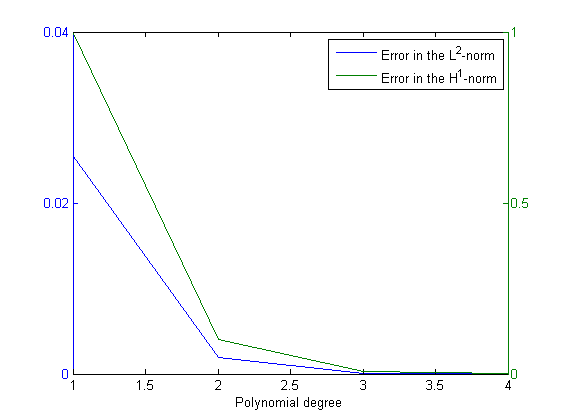
\includegraphics[width=0.65\textwidth]{fig/polyerrorf1_ref3.png}
\caption{Global error in the $L^2$- and $H^1$-norm as function of the polynomial degrees for the first example for $M = N = 1$.}
\label{error_polydegree_example1}
\end{figure}
As we can see, the plots reflect the expected behaviour, because the error decreases exponentially.
\subsubsection{Second Example}
Looking at fig. \ref{error_comparison}, we can see the comparison of the global error in the $H^1$-norm for the two different examples with fixed refinement level of three. Note that $M = N = 1$ holds for the first example.
\begin{figure}[h!]
  \centering      
  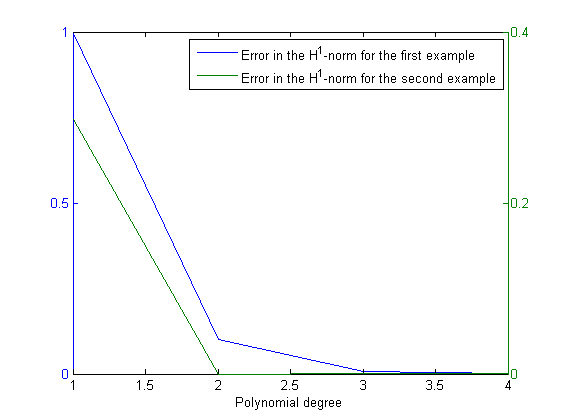
\includegraphics[width=0.65\textwidth]{fig/ComparisonH1error.png}
\caption{Global error in the $H^1$-norm as function of the polynomial degrees for the two different examples.}
\label{error_comparison}
\end{figure}
In fig. \ref{error_comparison} one can see that the global error in the $H^1$-norm for the second example is for polynomial degree of two zero. This can be explained by the fact, that the right-hand side in the second example is a polynomial of degree two.

\newpage
\section{The Condition Number of the Stiffness Matrix}
\subsection{Dependence on the Level of Refinement and on the Polynomial Degree}
It is very difficult to derive theoretical results on the dependence of the condition number of the stiffness matrix on the level of refinement and the polynomial degree. There are several reasons:
\begin{itemize}
\item The number of elements per row in the matrix depends on the geometry. It makes great differences if we choose triangles, rectangles etc. .
\item Furhtermore, depending on the angles in one element, each degree fo freedom might have another number of adjacent neighbour nodes.
\item Depending on the above two points, the number of adjacent neighbours additionally depends on the degree of the ansatz functions.
\end{itemize}
As a consequence, all three of these points determine the elements of the stiffness matrix so that it is more or less impossible to derive theoretical results except for special cases. \\
The results of some numerical experiments indicate that there is a dependence of the form
\begin{equation*}
\kappa = O \left( \left( \frac{1}{h} \right) ^{p+1} \right),
\end{equation*}
where $\kappa$ denotes the condition numer of the stiffness matrix.
\subsection{The CG-Method and the Condition Number}
Let $A \in \mathbb{R}^{n \times n}$ be the stiffness matrix of the Poisson problem and $x_0 \in \mathbb{R}^n$ any initial vector to the CG-method. Then it is known from numerical analysis that the error in the $k$-th iteration is extimated by
\begin{equation}
\Vert x_k - x^*\Vert_A \leq 2 \left( \frac{\sqrt{\kappa} - 1}{\sqrt{\kappa} +1} \right) ^k \Vert x_0 - x^*\Vert_A, \notag
\end{equation}
where $\kappa$ denotes the condition number of the stiffness matrix, $x^*$ the exact solution, $x_k$ the $k$-th iterate in the CG-method and 
\begin{equation}
\Vert x\Vert_A := \sqrt{x^T A x} \notag
\end{equation}
is the $A$-norm of $x \in \mathbb{R}^n$ (see e.g. \cite[Chap IV Theorem 3.7]{braess}). Let $\varepsilon > 0$ denote the given tolerance to the CG-method. Then we want that
\begin{equation}
\Vert x_k - x^*\Vert_A \leq 2 \left( \frac{\sqrt{\kappa} - 1}{\sqrt{\kappa} +1} \right) ^k \Vert x_0 - x^*\Vert_A \leq \varepsilon \Vert x_0 - x^*\Vert_A \notag
\end{equation}
holds and it follows
\begin{equation}
k \geq \frac{\log ( \frac{\varepsilon}{2})}{\log ( \frac{\sqrt{\kappa} - 1}{\sqrt{\kappa} +1}) }. \notag
\end{equation}

\section{Parallelization}
All content about laws on parallel performance can be found in \cite{weiss}.
\subsection{Speedup and Efficiency}
Let $T(P)$ the runtime of a parallel algorithm on $P$ processors and let $T_S$ the runtime of the best sequential implementation of the algorithm. Then the speedup $S(P)$ and the efficiency $E(P)$ are defined by
\begin{align}
S(P) := \frac{T_S}{T(P)}, \label{speedup}\\
E(P) := \frac{S(P)}{P}. \notag
\end{align}
The efficiency is a measure of the utilized capacity of the processors. In an ideal world we want $S(P) \approx P$ and $E(P) \approx 1$. In practise $T(1)$ is often used instead of $T_S$ and it holds $T(1) \geq T_S$. So for some algorithms one can obtain $S(P) > P$ and $E(P) > 1$ due to cache effects, data locality etc. . \\
When $T_S$ or $T(1)$ can not be determined because of the problem size the incremental speedup 
\begin{align*}
S_I(P) := \frac{T(\frac{P}{2})}{T(P)} \quad ( \leq 2)
\end{align*} 
is considered instead.

\subsection{Amdahl's Law}
When we parallelize an algorithm, we want to save runtime for the same problem size. But in practise most algorithms won't scale perfectly because they contain sequential parts which can not be parallelized. An estimation about the speedup that we can expect is given by Amdahl's law. \\
Let  $T(1)$ the time for the sequential run of the program. Let $f$ with $0 \leq f \leq 1$ the part of the program which is not parallelizable. Then it holds for the runtime $T(P)$ of the parallel execution on $P$ processors
\begin{align}
T(P) = f \cdot T(1) + \frac{1 - f}{P}T(1). \label{amdahl}
\end{align}
Inserting (\ref{amdahl}) into (\ref{speedup}) we obtain
\begin{align}
S(P) = \frac{T(1)}{T(P)} = \frac{1}{f + \frac{1-f}{P}}. \label{amdahlII}
\end{align}
Now, one can ask what happens if we increase the number of processors more and more? Do we get infinite speedup? Letting $P \to \infty$ in (\ref{amdahlII}) we see that the speedup saturates with limit
\begin{align*}
\lim_{P \to \infty} S(P) = \frac{1}{f}.
\end{align*}
So the maximal speedup is given by the sequential part of the program. \\
Amdahl's law is often beeing critisised because it does not consider the problem size $N$. If the sequential part of the program is independ on the problem size and only the parallel part depends on it then Amdahl's law is too pessimistic. Another approach that avoids this problem is the law by Gustafson.

\subsection{Gustafson's Law}
Let the number of processors $P$ fixed. Let $f(N)$ the sequential part of the algorithm for the problem size $N$. Furthermore, let $T(P) = 1$ normed. Then it holds:
\begin{align*}
T(P) = f(N) + (1 - f(N)), \quad T(1) = f(N) + (1 - f(N)) \cdot P, \\
S(P) = \frac{T(1)}{T(P)} = f(N) + (1 - f(N)) \cdot P
\end{align*}
where we used $T(P) = 1$ in the last equation. If it holds
\begin{align*}
\lim_{N \to \infty} f(N) = 0
\end{align*}
then we obtain
\begin{align*}
\lim_{N \to \infty} s(N) = P
\end{align*}
as desired. This is a realistic scenario for many problems.

\newpage
\appendix

\bibliography{tutorials_bib}
\bibliographystyle{plain}

\printindex

\end{document}
